\documentclass[border=0pt]{standalone}
\usepackage{graphicx,xcolor,tikz}
% https://tex.stackexchange.com/questions/128496/elegant-fractions-in-one-line
\newcommand{\uk}{\ensuremath{\bot}}
\begin{document}
    %\tdplotsetmaincoords{50}{130}
    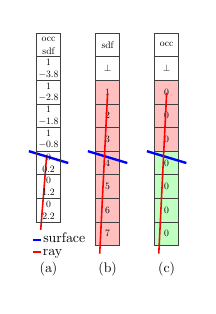
\begin{tikzpicture}
        \node at (0.5, 0.075) {\scalebox{.35}{$-0.8$}};
        \node at (0.5, 0.225) {\scalebox{.35}{$1$}};
        \node at (0.5, 0.375) {\scalebox{.35}{$-1.8$}};
        \node at (0.5, 0.525) {\scalebox{.35}{$1$}};
        \node at (0.5, 0.675) {\scalebox{.35}{$-2.8$}};
        \node at (0.5, 0.825) {\scalebox{.35}{$1$}};
        \node at (0.5, 0.975) {\scalebox{.35}{$-3.8$}};
        \node at (0.5, 1.125) {\scalebox{.35}{$1$}};
        \node at (0.5, 1.275) {\scalebox{.35}{sdf}};
        \node at (0.5, 1.425) {\scalebox{.35}{occ}};
    
        \draw[line width=0.1mm,black!75] (0.35, 0) rectangle (0.65,0.3);
        \draw[line width=0.1mm,black!75] (0.35, 0.3) rectangle (0.65,0.6);
        \draw[line width=0.1mm,black!75] (0.35, 0.6) rectangle (0.65,0.9);
        \draw[line width=0.1mm,black!75] (0.35, 0.9) rectangle (0.65,1.2);
        \draw[line width=0.1mm,black!75] (0.35, 1.2) rectangle (0.65,1.5);
    
        \draw[line width=0.3mm,blue] (0.25,0) -- (0.75,-0.15);
        \draw[line width=0.2mm,red] (0.4,-1) -- (0.475,-0.07);
        
        \draw[line width=0.1mm,black!75] (0.35, 0) rectangle (0.65,-0.3);
        \draw[line width=0.1mm,black!75] (0.35, -0.3) rectangle (0.65,-0.6);
        \draw[line width=0.1mm,black!75] (0.35, -0.6) rectangle (0.65,-0.9);
        
        \node at (0.5, -0.075) {\scalebox{.35}{$0$}};
        \node at (0.5, -0.225) {\scalebox{.35}{$0.2$}};
        \node at (0.5, -0.375) {\scalebox{.35}{$0$}};
        \node at (0.5, -0.525) {\scalebox{.35}{$1.2$}};
        \node at (0.5, -0.675) {\scalebox{.35}{$0$}};
        \node at (0.5, -0.825) {\scalebox{.35}{$2.2$}};
        
        \draw[line width=0.3mm,blue] (0.3, -1.125) -- (0.4, -1.125);
        \node at (0.7,-1.1) {\scalebox{.5}{surface}};
        
        \draw[line width=0.2mm,red] (0.3, -1.28) -- (0.4, -1.28);
        \node at (0.55,-1.3) {\scalebox{.5}{ray}};
        
        \node at (0.5, -1.5) {\scalebox{.5}{(a)}};
        
        \begin{scope}[shift={(0.75,0)}]            
            \draw[line width=0.1mm,black!75,fill=red!25] (0.35, 0) rectangle (0.65,0.3);
            \draw[line width=0.1mm,black!75,fill=red!25] (0.35, 0.3) rectangle (0.65,0.6);
            \draw[line width=0.1mm,black!75,fill=red!25] (0.35, 0.6) rectangle (0.65,0.9);
            \draw[line width=0.1mm,black!75] (0.35, 0.9) rectangle (0.65,1.2);
            \draw[line width=0.1mm,black!75] (0.35, 1.2) rectangle (0.65,1.5);
            
            \node at (0.5, 0.15) {\scalebox{.35}{$3$}};
            \node at (0.5, 0.45) {\scalebox{.35}{$2$}};
            \node at (0.5, 0.75) {\scalebox{.35}{$1$}};
            \node at (0.5, 1.05) {\scalebox{.35}{$\uk$}};
            \node at (0.5, 1.35) {\scalebox{.35}{sdf}};
            
            \draw[line width=0.1mm,black!75,fill=red!25] (0.35, 0) rectangle (0.65,-0.3);
            \draw[line width=0.1mm,black!75,fill=red!25] (0.35, -0.3) rectangle (0.65,-0.6);
            \draw[line width=0.1mm,black!75,fill=red!25] (0.35, -0.6) rectangle (0.65,-0.9);
            \draw[line width=0.1mm,black!75,fill=red!25] (0.35, -0.9) rectangle (0.65,-1.2);
            
            \node at (0.5, -0.15) {\scalebox{.35}{$4$}};
            \node at (0.5, -0.45) {\scalebox{.35}{$5$}};
            \node at (0.5, -0.75) {\scalebox{.35}{$6$}};
            \node at (0.5, -1.05) {\scalebox{.35}{$7$}};
            
            \draw[line width=0.3mm,blue] (0.25,0) -- (0.75,-0.15);
            \draw[line width=0.2mm,red] (0.4,-1.3) -- (0.5,0.74);
            
            \node at (0.5, -1.5) {\scalebox{.5}{(b)}};
        \end{scope}
        
        \begin{scope}[shift={(1.5,0)}]            
            \draw[line width=0.1mm,black!75,fill=red!25] (0.35, 0) rectangle (0.65,0.3);
            \draw[line width=0.1mm,black!75,fill=red!25] (0.35, 0.3) rectangle (0.65,0.6);
            \draw[line width=0.1mm,black!75,fill=red!25] (0.35, 0.6) rectangle (0.65,0.9);
            \draw[line width=0.1mm,black!75] (0.35, 0.9) rectangle (0.65,1.2);
            \draw[line width=0.1mm,black!75] (0.35, 1.2) rectangle (0.65,1.5);
            
            \node at (0.5, 0.15) {\scalebox{.35}{$0$}};
            \node at (0.5, 0.45) {\scalebox{.35}{$0$}};
            \node at (0.5, 0.75) {\scalebox{.35}{$0$}};
            \node at (0.5, 1.05) {\scalebox{.35}{$\uk$}};
            \node at (0.5, 1.35) {\scalebox{.35}{occ}};
            
            \draw[line width=0.1mm,black!75,fill=green!25] (0.35, 0) rectangle (0.65,-0.3);
            \draw[line width=0.1mm,black!75,fill=green!25] (0.35, -0.3) rectangle (0.65,-0.6);
            \draw[line width=0.1mm,black!75,fill=green!25] (0.35, -0.6) rectangle (0.65,-0.9);
            \draw[line width=0.1mm,black!75,fill=green!25] (0.35, -0.9) rectangle (0.65,-1.2);
            
            \node at (0.5, -0.15) {\scalebox{.35}{$0$}};
            \node at (0.5, -0.45) {\scalebox{.35}{$0$}};
            \node at (0.5, -0.75) {\scalebox{.35}{$0$}};
            \node at (0.5, -1.05) {\scalebox{.35}{$0$}};
            
            \draw[line width=0.3mm,blue] (0.25,0) -- (0.75,-0.15);
            \draw[line width=0.2mm,red] (0.4,-1.3) -- (0.5,0.74);
            
            \node at (0.5, -1.5) {\scalebox{.5}{(c)}};
        \end{scope}
    \end{tikzpicture}
\end{document}